\section{AES Overview}

AES is a \textit{Symmetric Block Cipher} operating on \textbf{128-bit data blocks}
and supporting three different key sizes (128/192/256-bit) according to the desired
security level.

As many block ciphers, it processes its internal \textit{state} (Figure \ref{fig:state}), initialized either with the
\textit{plaintext} or \textit{ciphertext}, in several rounds. They all share the same
structure safe for the last (first) one during encryption (decryption).

\begin{figure}[h]
  \centering
  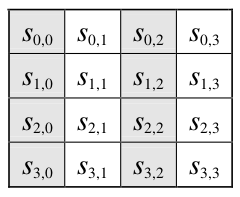
\includegraphics[width=0.2\textwidth]{figures/aes_state}
  \caption{Logical depiction of the AES internal state}
  \label{fig:state}
  \centering
\end{figure}

The round is structured as follows:
\begin{enumerate}
  \item \texttt{SubBytes} implements the non-linear layer (confusion) of the cipher. It
operates a 8-bit to 8-bit transformation (usually implemented via simple lookups)
based on GF(2\textsuperscript{8}) inverse calculation
  \item \texttt{ShiftRows} performs the first step of the linear diffusion layer just
by rotating the bytes on the same row of the state
  \item \texttt{MixColumns} performs the second step of the linear diffusion layer
by performing GF(2\textsuperscript{8}) multiplications by constants
  \item \texttt{AddRoundKey} is a simple XOR with the round-key, and it's the secret
dependent phase of the round
\end{enumerate}

\begin{figure}[h]
  \centering
  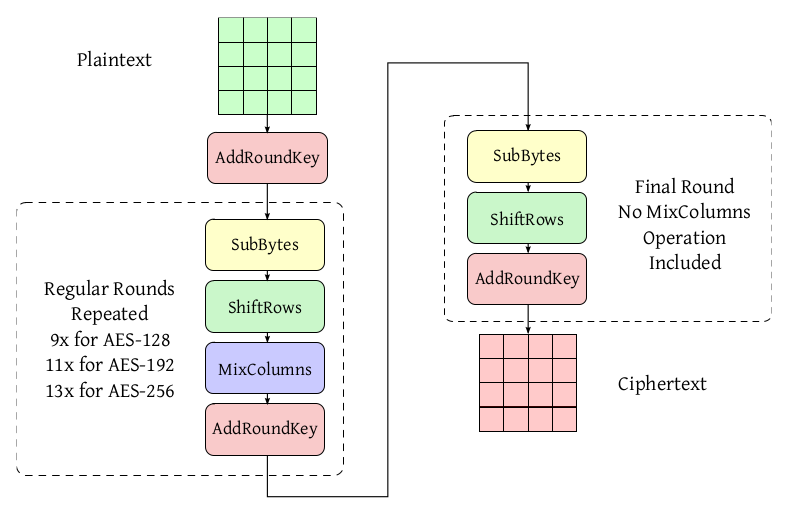
\includegraphics[width=0.6\textwidth]{figures/aes_encryption}
  \caption{AES encryption operation}
  \label{fig:enc}
\end{figure}
The overall encryption flow is depicted in Figure \ref{fig:enc}.

\subsection{From Sboxes to Tboxes}

The main intuition behind the Tbox-based implementation is that some of the round
transformations of the AES cipher commute.

In particular, \texttt{SubBytes} and \texttt{ShiftRows} can be swapped immediately.
This brings \texttt{SubBytes} and \texttt{MixColumns} close together. Tboxes are
basically the result of merging these two phases. Instead of mapping state-bytes
to Sboxes and then transforming them through \texttt{MixColumns}, we
precompute the results and store them in a ROM for later use.

Each state-byte has to be looked-up in both of the approaches. However, while an Sbox maps
it to an 8-bit value, a Tbox outputs a 32-bit word. At the cost of 4x ROM space, we can skip
all the circuitry and latency associated to the \texttt{MixColumns} stage.

\texttt{MixColumns} operates on a 32-bit \textit{state column} seen as a 4-byte
column vector $\begin{bmatrix} s_{0} , & s_{1} , & s_{2} , & s_{3} \end{bmatrix}$. The resulting transformation is:


\begin{gather}
  \begin{bmatrix} % input state bytes...
    s_{0}' \\ s_{1}' \\ s_{2}' \\ s_{3}'
  \end{bmatrix}
  =
  \begin{bmatrix}
    02 & 03 & 01 & 01 \\
    01 & 02 & 03 & 01 \\
    01 & 01 & 02 & 03 \\
    03 & 01 & 01 & 02
  \end{bmatrix}
  \begin{bmatrix} % input state bytes...
    s_{0} \\ s_{1} \\ s_{2} \\ s_{3}
  \end{bmatrix}
  =
  \begin{bmatrix}
    02 \\ 01 \\ 01 \\ 03
  \end{bmatrix}
  \begin{bmatrix} s_{0} \end{bmatrix} \oplus
  \begin{bmatrix}
    03 \\ 02 \\ 01 \\ 01
  \end{bmatrix}
  \begin{bmatrix} s_{1} \end{bmatrix} \oplus
  \begin{bmatrix}
    01 \\ 03 \\ 02 \\ 01
  \end{bmatrix}
  \begin{bmatrix} s_{2} \end{bmatrix} \oplus
  \begin{bmatrix}
    01 \\ 01 \\ 03 \\ 02
  \end{bmatrix}
  \begin{bmatrix} s_{3} \end{bmatrix}
\end{gather}

The multiplication of each constant column vector against a state byte defines
a Tbox, which can be thus precalculated for each of the 256 values of the initial
Sbox.
It is not necessary to store the 4 Tboxes separately, as each one of them can be
computed via a simple byte rotation.
In particular, the original Tbox directly maps the state-bytes of the first row of
the AES state. The Tboxes for the second/third/fourth row are obtained by rotating
the original Tbox 1/2/3 bytes on the right.

Since \texttt{ShiftRows} is a simple rotation of the state-bytes on the same row of
the AES state -- which implies a trivial rewiring in hardware -- the round structure
of the AES cipher can be squashed in a single operation.

Let the AES state be the one in Figure \ref{fig:state}.
$s^k_{i,j}$ is a single state byte at the \textit{k-th} round of the cipher.
Let $ TBOX(s,i) $ be a function that maps an 8-bit value $s$ to a 32-bit word that
is rotated $i$ bytes to the right.
Finally, let $S_i^k$ with $i=0,1,2,3$ be the \textit{i-th} column of the 128-bit
state at the \textit{k-th} round and $R^k_i$ the \textit{i-th} column of the \textit{k-th} round-key.
Then:
\begin{equation}
  \begin{align*}
    S_i^k\quad =\quad TBOX(s^{k-1}_{0,i},0)\quad \oplus\quad TBOX(s^{k-1}_{1,i+1\bmod4},1)\quad \oplus \\
      TBOX(s^{k-1}_{2,i+2\bmod4},2)\quad \oplus\quad TBOX(s^{k-1}_{3,i+3\bmod4},3)\quad \oplus\quad R^k_i
  \end{align*}
  \label{eq:tbox}
\end{equation}

Since we can perform all the Tbox lookups parallel given enough (i.e. 16) ROMs,
and that the operations are simple XORs, this version of the AES cipher is particularly suitable
for a fast hardware implementation.
The final round, that skips the \texttt{MixColumns} transformation, just uses the
output of the original Sboxes.

\subsection{Inverse Cipher with Tboxes}
\label{sec:inv_tbox}

The sequence of operations of the AES decryption round is the inverse of the encryption:
\texttt{AddRoundKey}, \texttt{InvMixColumns}, \texttt{InvShiftRows}, \texttt{InvSubBytes}.
While \texttt{InvShiftRows} and \texttt{InvSubBytes} still commute, the latter is a non-linear
operation and thus doesn't commute with the linear permutation layer, that is, \texttt{InvMixColumns}.

However, since \texttt{InvMixColumns} is linear, it can be swapped with \texttt{AddRoundKey} given
that also the round key undergoes the \texttt{InvMixColumns} transformation:
\begin{equation}
  InvMixColumns(S^k_i\quad \oplus\quad R^k_i)\quad = \quad InvMixColumns(S^k_i)\quad \oplus\quad InvMixColumns(R^k_i)
  \label{eq:tbox}
\end{equation}
By employing an inverse key schedule in which all the round keys, but the first and the
last, have gone through the \texttt{InvMixColumns}, it is possible to obtain the exact same
execution flow of the encryption, safe for:
\begin{enumerate}
  \item alternate round keys, that need to be stored and incur in a 2x space overhead
  \item inverse Tboxes, that are crafted in the same exact way as the direct one,
by multiplying the constant vector
$\begin{bmatrix} 0E , & 09 , & 0D , & 0B \end{bmatrix}$ and
the \texttt{InvSubBytes} outputs
\end{enumerate}

This solution, adopted in our AES core, allows to totally reuse the encryption datapath
for decryption by just selecting the alternate round key and the inverse
Tbox values instead of the direct ones.
